\subsection{Detectores de posición y velocidad.}

    % Autoridad > derecho limitado a una porcion
    % Claridad > autoridad no ambigua
    % Anticipacion > avisar con antelacion
    % Granularidad > rutas cortas y funcionales
    % Terminalidad > avisar fin de via
    % Infraestructura > avisar de infraestructura
    % No bloqueo > circulacion fluida
    
    En la Sección \ref{sec:detectors} definimos dos elementos ferroviarios utilizados para detectar la posición de una formación: los contadores de ejes y los circuitos de vía. Adicionalmente, los contadores de ejes se utilizan para calcular la velocidad de la formación. Es claro que, para no alterar la medición de velocidad, no tiene sentido detener la marcha de la formación próximo a un contador de ejes y por lo tanto el principio de anticipación ($P_3$) no se aplica. Adicionalmente, los contadores de ejes no representan un peligro para la formación, al encontrarse en la cara interna de la vía no es posible para una formación colisionar con ellos, por lo que cubrimos el principio de infraestructura ($P_6$) sin utilizar ninguna señal. En conclusión, el RNA no requiere agregar ninguna señal asociada a los contadores de ejes.

    Utilizamos a las junturas como los elementos divisorios entre los circuitos de vía a los cuales aplicaremos el principio de antelación y autoridad ($P_1$). Por el principio de antelación, las señales deben colocarse antes de cada juntura para indicar con suficiente tiempo si se puede proseguir la marcha o no hacia una nueva sección. Además, como solo una formación a la vez puede ocupar cada circuito de vía, el principio de autoridad ($P_1$) se aplica para restringir el acceso a las próximas secciones de encontrarse ocupadas. Finalmente, por el principio de no bloqueo ($P_7$), podemos asumir que no tiene sentido detener la marcha de las formaciones en secciones muy pequeñas, incluso mas pequeñas que una formación, por lo que solo se aplicaran señales en secciones mayores a un tamaño determinado.
    
    En el Algoritmo \ref{alg:RJ} se define la asignación de señalamientos para los contadores de ejes y circuitos de vía limitados por las junturas. El parámetro de largo mínimo para la sección puede ser modificado por el operador, pero es único para toda la red. De esta forma nos aseguramos, además, que redes ferroviarias de gran tamaño pero sin demasiados elementos ferroviarios pueda tener señalamiento cada cierta cantidad de metros o kilómetros. Ya que toda red ferroviaria esta constituida por rieles que presentan junturas cada ciertas distancias para evitar que la expansión térmica provoque descarrilamientos.

    \begin{algorithm}[hbt!]
        \caption{Algoritmo de generación de señalamiento para Axle Counters y Rail Joints}\label{alg:RJ}
        \DontPrintSemicolon
        %\SetAlgoLined
        \SetNoFillComment
        \LinesNotNumbered 
        \If { netElement WITH AxleCounters }
        {
            // Do nothing
        }
        \For { netElement WITH RailJoints }
        {
            Track.Length = Length ( between RailJoints )\;
            \If { Track.Length $>$ FIXED\_LENGTH }
            {
                [Signals] $\gets$ ADD circulation signal $\gg\gg$\;
                [Signals] $\gets$ ADD circulation signal $\ll\ll$\;
            }
        }
        \KwResult{[Signals]} 
    \end{algorithm} 

    Aplicando el Algoritmo \ref{alg:RJ} a un sistema de tres vías paralelas se obtiene un resultado como el ilustrado en la Figura \ref{fig:signal_detector}. La vía superior presenta un contador de ejes, la vía intermedia dos circuitos de vía, uno corto y uno largo. La vía inferior presenta dos circuitos de vía, ambos de larga longitud.
    
    \begin{figure}[h!]
        \centering
        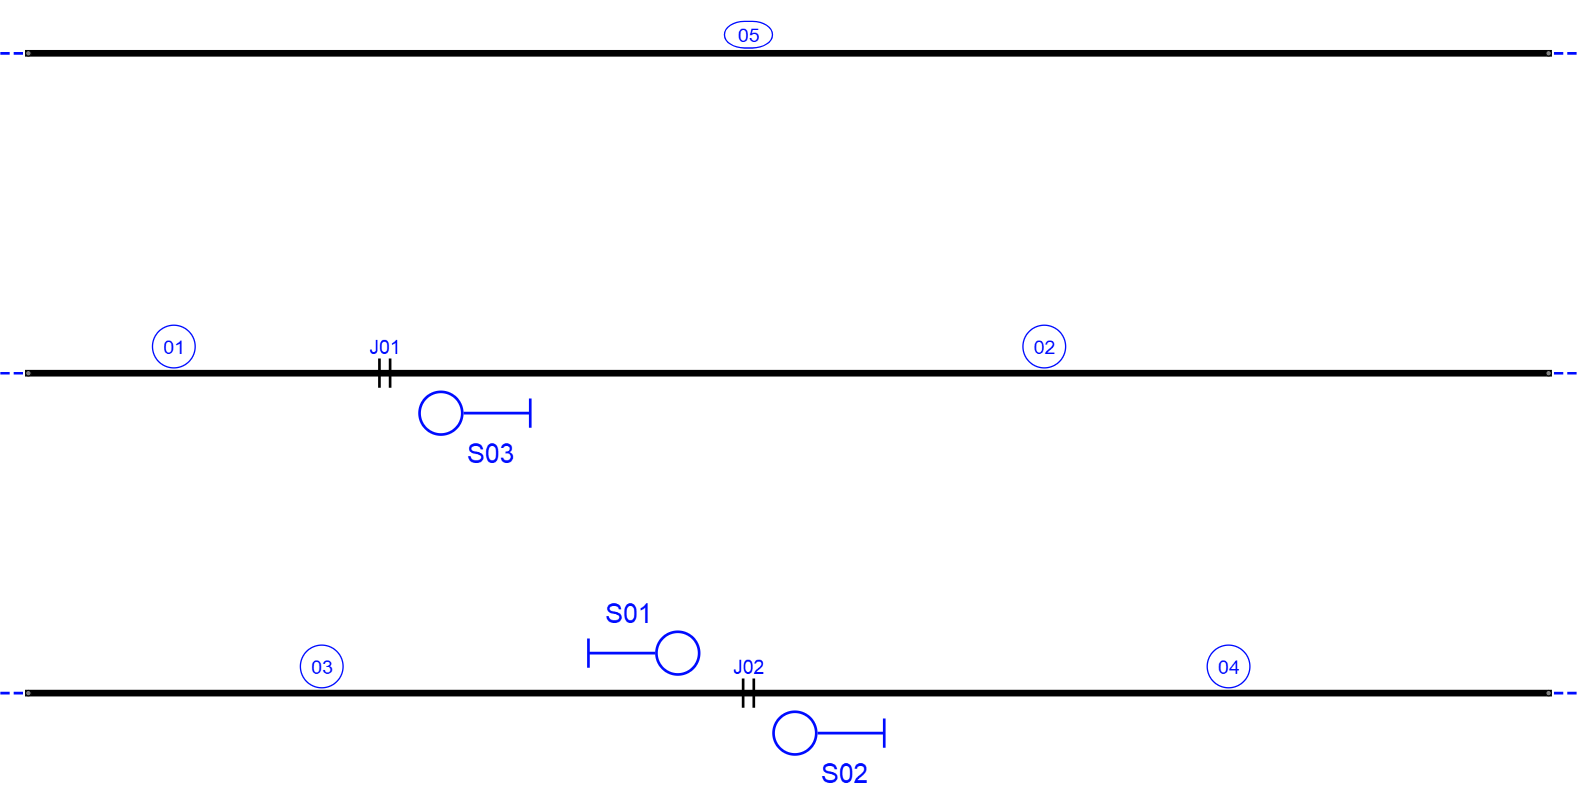
\includegraphics[width=1\textwidth]{Figuras/detectores.PNG}
        \centering\caption{Señalamiento generado para contadores de ejes y circuitos de vías.}
        \label{fig:signal_detector}
    \end{figure}

    La vía superior incluye al contador de ejes 05 y no se le asigna ninguna señal. La vía intermedia tiene dos secciones, la primera es la correspondiente al circuito de vía 01 y no se le asigna una señal al ser muy corta, la segunda es la correspondiente al circuito de vía 02 y se le asigna la señal S03 antes de la juntura J01. La señal S03 se utiliza para detener la formación que transita de derecha a izquierda antes de ingresar a la sección del circuito de vía 01 y reiniciar la marcha si esta última se encuentra desocupada. Finalmente, las señales S01 y S02 se asignan antes de la juntura J02 para poder transitar desde la sección del circuito de vía 03 a la sección del circuito de vía 04 y viceversa.